\documentclass[tikz,border=5mm]{standalone}
\usetikzlibrary{calc,intersections}
\begin{document}
	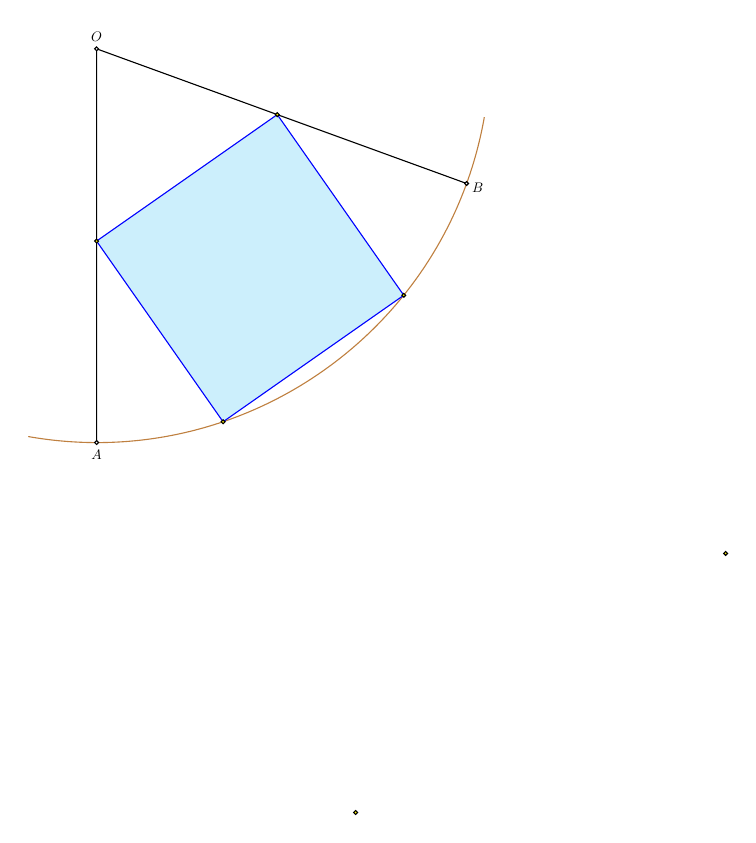
\begin{tikzpicture}
		\def\r{5} \def\go{70}
		\path(0:0) coordinate(O) (-90:\r)coordinate(A)
		($(O)!1!\go:(A)$)coordinate (B) ($(B)!1!90:(A)$)coordinate (C)($(C)!1!90:(B)$)coordinate (D);
		\draw[name path=cung,brown] (-100:\r) arc (-100:\go-80:\r);
		\path[name path=OD] (D)--(O);
		\path[name path=OC] (C)--(O);
		\path[name intersections={of=cung and OD,by=E}];
		\path[name intersections={of=cung and OC,by=F}];
		\path ($(F)!1!-90:(E)$)coordinate (G)($(G)!1!-90:(F)$)coordinate (H);
		\draw[blue,fill=cyan!20] (E)--(F)--(G)--(H)--cycle;
		\draw (A)--(O)--(B);
		\foreach \x in {C,D,E,F,G,H}\draw[fill=yellow] (\x) circle (.7pt);
		\foreach \x/\g in {O/90,A/-90,B/-20}\draw[fill=white] (\x) circle (.7pt)+(\g:.15)node[scale=.5]{$\x$};
	\end{tikzpicture}
\end{document}